\section{Shop}
\label{shop}

\begin{figure}[ht]
	\centering
  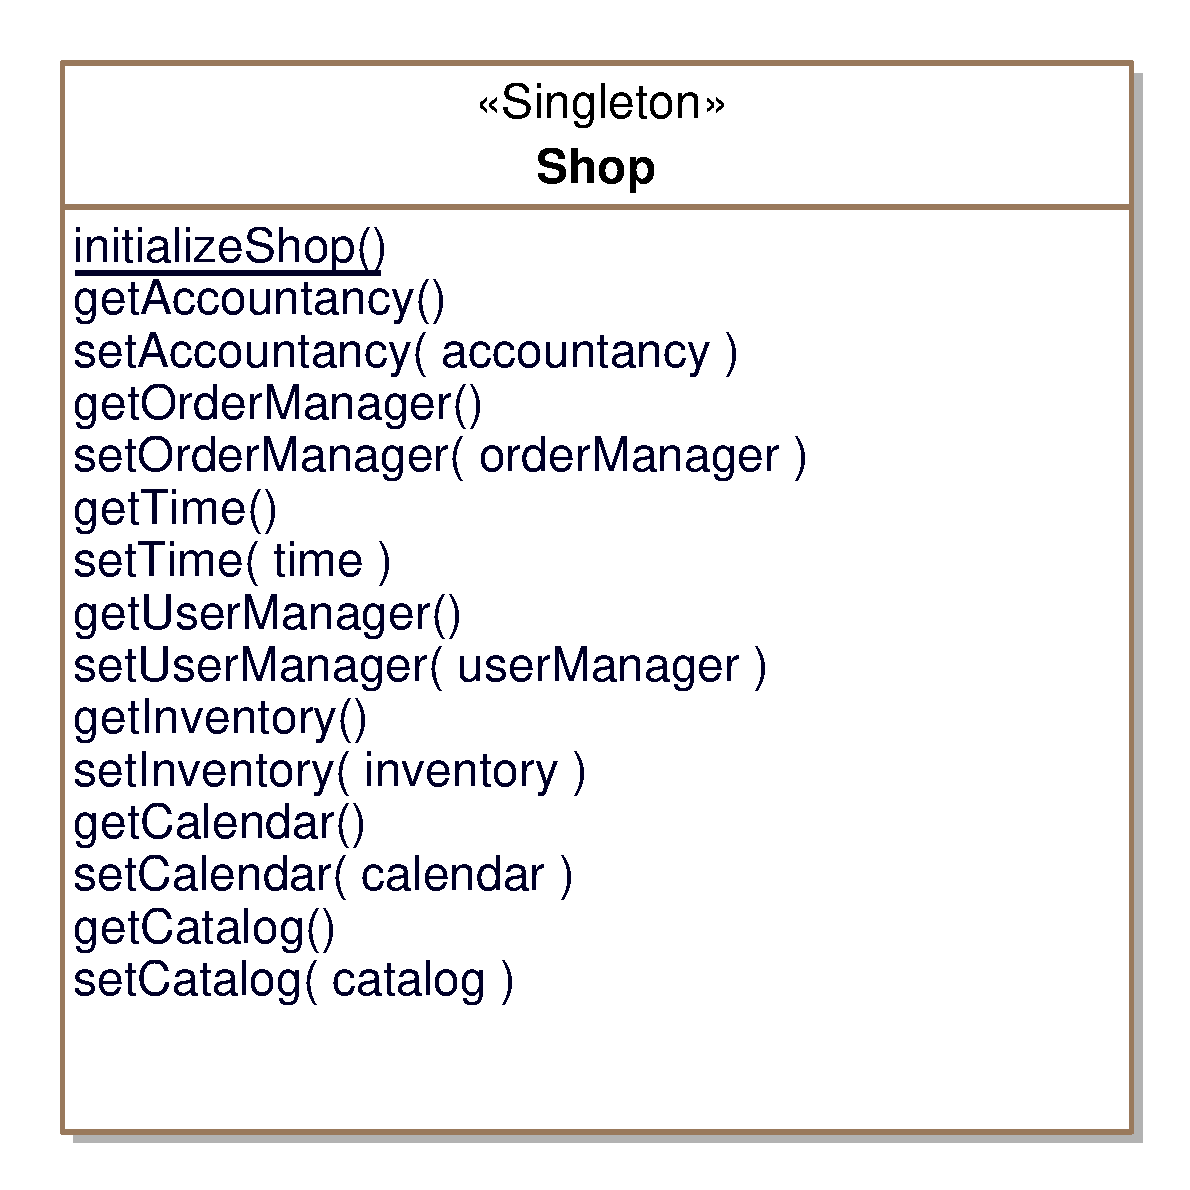
\includegraphics[width=0.65\textwidth]{images/Shop_Overview.eps}
	\label{shop_overview}
	\caption{Shop - Class Overview}
\end{figure}

%\subsection{\code{Shop} - Starting your SalesPoint-application}
\code{Shop} is a central class in \salespoint{}; it holds references to all manager interfaces and a reference to the \code{Time} interface.
There are six manager interfaces in \salespoint{}: Accountancy, Calendar, Catalog, Inventory, OrderManager and UserManager.
Other classes use the \code{Shop} to access the manager interfaces, for example \code{Order.completeOrder()} uses \code{Shop.INSTANCE.getInventory()} for product removal.
\code{PersistentCalendar} uses \code{Shop.INSTANCE.getTime()} for time based operations.
There is also a convenience method to minimize boilerplate code \code{Shop.initializeShop()}; it is used for setting all managers of \code{Shop} to Salespoints persistent class implementations and the time to \code{DefaultTime}.
\code{Shop} is implemented as singleton.
